% Create a Table of Contents in Beamer
\documentclass{beamer}
% Theme choice:
\usetheme{Singapore}
\usecolortheme{whale}
\setbeamercolor{titlelike}{fg=blue,bg=white}
\setbeamercolor{frametitle}{fg=blue,bg=white}
\setbeamertemplate{frametitle}[default][left]
\setbeamertemplate{navigation symbols}{}

\usepackage{graphicx}
\usepackage{amsmath}
\usepackage{amsfonts}
\usepackage{amssymb}
\usepackage{amsthm}

% Title page details: 
\title{Chapter 2: Regression for binary outcomes} 
\author{Taylor Okonek \& Charlie Wolock}
\date{\today}



\begin{document}
	% Title page frame
	\begin{frame}
	\titlepage 
\end{frame}

\begin{frame}{Learning objectives}
	By the end of Chapter 2, you should be able to: 
	\begin{itemize}
		\item Distinguish between probability and odds and know how to calculate each in \texttt{R}
		\item Describe the measures of association used for binary outcomes and exposures of interest
		\item Formulate a regression model, given a scientific or statistical question about a binary outcome
		\item Interpret the coefficients (along with confidence intervals and p-values) of a regression model for a binary outcome
		\item Describe how (and why) logistic regression interpretation changes when we have data from a case-control study
		\item Use \texttt{R} to fit a logistic regression model and produce supporting figures/tables
	\end{itemize}
\end{frame}

% Outline frame
\begin{frame}{Outline}
\tableofcontents
\end{frame}

\AtBeginSection[ ]
{
\begin{frame}{Outline}
\tableofcontents[currentsection]
\end{frame}
}

% Presentation structure
\section{Binary outcomes}

% quantitative outcomes from ch1
\begin{frame}{Recall: Variable type}
	In Chapter 1, we ask scientific questions involving quantitative outcomes: those that have a fundamentally numeric quality: 
	\\~\
	
	\textcolor{red}{Insert examples from Chapter 1.}
\end{frame}

% binary variable examples
\begin{frame}{Recall: Variable type}
Binary variables are a type of \textcolor{blue}{categorical} variable with two possible categories. We often implicitly think of them in a 0-1 sense, but they don't have actual numeric value. 
\\~\

Examples we often see in biomedical research: 
\begin{itemize}
	\item Type I diabetes (presence/absence)
	\item Surgery complications (occurred/did not occur)
	\item Smoking (yes/no)
	\item Mortality prior to age 5 (occurred/did not occur)
	\item COVID status (positive/negative)
\end{itemize}
\end{frame}

% binary variable scientific questions
\begin{frame}{Scientific questions about binary variables}
	Questions we could ask about these variables include
	\begin{itemize}
		\item Are variants in the HLA-DRB1 gene associated with \textcolor{blue}{Type I diabetes}? 
		\item Are \textcolor{blue}{surgery complications} after upper endoscopy associated with who (anesthesiologist vs nurse) performed the sedation?
		\item Is the use of e-cigarettes associated with \textcolor{blue}{smoking}?
		\item \textcolor{red}{Insert question from Taylor here}
		\item Is Vitamin D intake associated with the risk of \textcolor{blue}{testing positive for COVID}?
	\end{itemize}
\end{frame}

\begin{frame}{Scientific questions about binary variables}
	One specific question that has been the subject of much study is 
	\begin{itemize}
		\item Is Type A behavior associated with risk of \textcolor{blue}{coronary heart disease} (CHD)?
	\end{itemize}
	\vspace{0.7cm}
	Type A behavior is a concept that was developed by cardiologists in the 1950s, and is characterized by being competitive, ambitious, work-driven, and time-conscious. The doctors who identified this ``personality type" thought it might be associated with the risk of CHD, and many studies investigated this association. 
\end{frame}

\begin{frame}{The WCGS Study}
	The Western Collaborative Group Study (WCGS) was designed in order to investigate a possible link between Type A behavior and CHD, and to develop a \textcolor{blue}{risk prediction} framework to select patients for intervention in order to decrease risk of CHD. 
	\\ ~\ 
	
	\textbf{Study description}: 3154 men aged 39-59 in California with no CHD history were enrolled in 1960 and 1961, subjected to a medical examination and history, and re-examined annually for interim cardiovascular history. The primary outcome was angina pectoris (chest pain due to heart disease). 
\end{frame}

\begin{frame}{Activity: Study design}
	Discuss with a partner: Based on the description below, what category of study was WCGS?
	\\ ~\
	
	\textbf{Study description}: 3154 men aged 39-59 in California with no CHD history were enrolled in 1960 and 1961, subjected to a medical examination and history, and re-examined annually for interim cardiovascular history. The primary outcome was angina pectoris (chest pain due to heart disease). 
\end{frame}

\begin{frame}{Recall: summarizing a binary variable}
	Let's think about Type A behavior  and CHD. 
	\\ ~\ 
	
	We can talk about the \textcolor{blue}{probability} of experiencing CHD among those with Type A behavior ($p_A$) and the probability of experiencing CHD among those without Type A behavior ($p_B$).
	\begin{itemize}
		\item Generally, ``probability," ``risk," ``proportion" refer to the same quantity.
	\end{itemize}
	\textcolor{blue}{Odds} are defined as $\frac{p}{1-p}$.
	\begin{itemize}
		\item Odds of diabetes with mutation: $\frac{p_A}{1-p_A}$
		\item Odds of diabetes with wild-type: $\frac{p_B}{1-p_B}$
	\end{itemize}
\end{frame}

\begin{frame}{Recall: summarizing a binary variable}
Probability:
\begin{itemize}
	\item Takes values in $[0,1]$.
	\item Generally more intuitive than odds. 
	\item In some study designs, are impossible to estimate! (More on this later.)
\end{itemize}
Odds:
\begin{itemize}
	\item Take values in $(0,\infty)$.
	\item Are less intuitive for most people (unless you do a lot of betting).
	\item Can be estimated from most common biomedical study designs. 
\end{itemize}
\end{frame}

\begin{frame}{Measures of association}
	We can now describe the \textcolor{blue}{probability} or \textcolor{blue}{odds} of having CHD among those with Type A behavior and those without. 
	\\ ~\
	
	\textbf{Scientific question:} Is exhibiting Type A behavior \textcolor{red}{associated} with CHD? 
	\\ ~\
	
	In order to do statistics, we need to clarify what \textcolor{red}{associated} means for binary variables.
\end{frame}

\begin{frame}{Measures of association}
Equal probabilities: If $p_m = p_w$, then
	\begin{itemize}
		\item[] $p_A - p_B = 0$ (\textcolor{red}{risk difference}) \quad \quad \quad $\frac{p_A}{p_B} = 1$ (\textcolor{red}{relative risk})
	\end{itemize}
	\vspace{0.8cm}
Equal odds: If $\frac{p_A}{1-p_A} = \frac{p_B}{1-p_B}$, then
	\begin{itemize}
		\item[] $\frac{\frac{p_A}{1-p_A}}{\frac{p_B}{1-p_B}}=1$ (\textcolor{red}{odds ratio})
	\end{itemize}
\vspace{0.8cm}
These are the three most common measures of association for binary outcomes. 
\end{frame}

\begin{frame}{Measures of association}
When we are approaching a scientific question about association, we need to think about
\begin{itemize}
	\item \textcolor{blue}{Summary measure:} Probability or odds
	\item \textcolor{red}{Contrast:} Difference or ratio
\end{itemize}
\vspace{0.5cm}
In our running example:
\begin{itemize}
	\item Is there a \textcolor{red}{difference} in the \textcolor{blue}{probability} of CHD between people with Type A behavior and those without?
	\item Is the \textcolor{red}{ratio} of \textcolor{blue}{probabilities} of CHD comparing people with and without Type A behavior equal to 1?
	\item Is the \textcolor{red}{ratio} of \textcolor{blue}{odds} of CHD comparing people with and without a Type A behavior equal to 1?
\end{itemize}
\end{frame}

\begin{frame}{Moving toward statistical inference}
	The full process:
	\begin{enumerate}
		\item Ask a scientific question: Is Type A behavior associated with CHD?
		\item Translate to a statistical question: Is there a \textcolor{red}{difference} in the \textcolor{blue}{probability} of CHD between people with Type A behavior and those without?
		\item Define a parameter: e.g. risk difference, odds ratio
		\item Take a sample: Think back to what we know about study design!
		\item Perform inference: 
		\begin{itemize}
			\item Calculate a statistic based on our sample
			\item Quantify uncertainty: confidence interval
			\item Perform a hypotehsis test: p-value
		\end{itemize}
	\end{enumerate}
\end{frame}



%% Linear regression
\section{Linear regression with binary outcomes}
\begin{frame}
	\frametitle{SECTION 2: LINEAR REGRESSION WITH BINARY OUTCOMES}
	
	% Learning objectives
	By the end of this section, you should be able to:
	\begin{itemize}
		\item Interpret linear regression coefficients when the outcome $Y$ is binary
		\item Write a summary of results from a linear regression analysis with a binary outcome
		\item List at least one advantage and one disadvantage of using linear regression with a binary outcome
	\end{itemize}
\end{frame}
\begin{frame}
	\frametitle{Simple linear regression with a binary outcome}
	Can we use linear regression to look at the association between an exposure and a binary outcome? Yes!
	\\ ~\
	
	A simple linear regression model: $E[Y \mid X] = \beta_0 + \beta_1 X$.
	\begin{footnotesize}
		\begin{itemize}
			\item Recall: $E[Y \mid X]$ is the \textcolor{blue}{\textit{expected value}} (average) of $Y$ given $X$ 
		\end{itemize}
	\end{footnotesize}
	\pause
	What's the average of a binary variable $Y$? \pause \textit{It's the probability that $Y$ equals 1!} $\left(\text{i.e., } E[Y] = \text{P}(Y=1)\right)$ \pause
	
	\begin{itemize} \itemsep +12pt
		\item[] $Y = \{ 0, 0, 1, 0, 1, 1, 0, 0, 1, 1 \}$ \pause
		\item[] $\bar{Y} = \frac{0 + 0 + 1 + 0 + 1 + 1 + 0 + 0 + 1 + 1}{10} = \frac{1}{2}$ \pause
		\item[] $\hat{p} = \hat{\text{P}}(Y=1) = \frac{5}{10} = \frac{1}{2} $
	\end{itemize}
\end{frame}

\begin{frame}
	\frametitle{Simple linear regression with binary outcomes}
	\textbf{Discuss with your neighbor:} 
	\\ ~\ 
	
	% recall activity
	Suppose we fit the simple linear regression model $$E[Y \mid X] = \beta_0 + \beta_1 X,$$ where our outcome $Y$ is binary.
	
	What is the interpretation for the coefficients in this model?
	
	\begin{enumerate}
			\item $\beta_0$
			\item $\beta_1$
		\end{enumerate} 
\end{frame}

% linear regression: diabetes vs sex
\begin{frame}
	\frametitle{Simple linear regression: Type A personality and CHD}
	\vspace{-0.5cm}
	In our \texttt{wcgs} dataset, \texttt{chd} is a binary variable indicating CHD over follow-up, and \texttt{tabp} is a binary variable indicating Type A behavior. 
	\\ ~\
	
	We can fit the linear regression model $E[\texttt{chd} \mid \texttt{tabp}] = \beta_0 + \beta_1\texttt{tabp} $.
	
	How do we interpret the regression coefficients? \vspace{-0.2cm}
	
	\begin{itemize}
		\item \color{blue} $\beta_0$: \pause the probability of CHD among those without Type A behavior \pause \color{black}\vspace{-0.2cm}
		\item[] \ \ \begin{scriptsize} (the average value of $C$ among those with $\texttt{tabp} = 0$) \end{scriptsize} \pause
		\item \color{blue} $\beta_1$: \pause the difference in probability of CHD between those with and without Type A behavior \pause \color{black} \vspace{-0.2cm}
		\item[] \ \ \begin{scriptsize}(the difference in average value of $C$ between $A\texttt{tabp} = 1$ and $\texttt{tabp} = 0$ groups) \pause \end{scriptsize}
	\end{itemize}
	
	\vspace{-0.2cm}
	To answer our statistical question \begin{small}\textit{(is there a difference in probability of CHD between Type A and others?)}\end{small} we just need to look at $\beta_1$!
\end{frame}

\begin{frame}{Simple linear regression: Type A personality and CHD}
	What does this example tell us? 
	\\ ~\
	
	In Chapter 1, we talked about differences in means. Nothing has changed!
	\\ ~\

	For binary outcomes: difference in means $=$ difference in probabilities.
\end{frame}

\begin{frame}{Multiple linear regression with binary outcomes}
	Everything we know about multiple linear regression extends to binary outcomes. 
	\\ ~\
	
	Linear regression model with a binary outcome: $$E[Y|X_1,\cdots,X_p] = \beta_0 + \beta_1 X_1 + \beta_2X_2 + \cdots \beta_p X_p$$ $$P[Y=1|X_1,\cdots,X_p] = \beta_0 + \beta_1 X_1 + \beta_2 X_2 + \cdots \beta_p X_p$$
	
	\color{blue} Interpretation: \color{black}
	\begin{itemize} 
		\item $\beta_0$: \pause probability that $Y=1$ when $X_1 = 0, \cdots X_p = 0$
		\item $\beta_1$: \pause difference in probability that $Y=1$ comparing two groups that differ by one unit in $X_1$ but are the same with respect to $X_2,\cdots,X_p$ 
		\item ...
	\end{itemize}
\end{frame}

\begin{frame}{Linear regression with binary outcomes: inference}
	\vspace{-1.5cm}
	\begin{align*} 
		E[Y|X_1,\cdots,X_p] = \beta_0 + \beta_1 X_1 + \beta_2 X_2 + \cdots \beta_p X_p 
	\end{align*}
	
	\vspace{-0.2cm}
	\color{blue} Inference:  \color{black}
	\begin{itemize}
		\item Identify the regression coefficient of interest, $\beta$. \pause % which one(s) answer(s) our scientific Q?
		\item Report an estimate of $\beta$, and interpret: \textit{We estimate that the difference in probabilities between two groups...} \pause
		\item Report a 95\% confidence interval for $\beta$, and interpret: \textit{Based on a 95\% confidence interval, this observed difference in probabilities would not be judged unusual if...} \pause
		\item Report the p-value from a hypothesis test of $H_0: \beta = 0$: \textit{These data provide evidence to suggest that this difference in probabilities is (is not) significantly different from zero ($p =$...).} \pause
		\item Add a conclusion relating back to our scientific question
	\end{itemize}
	% they'll fill in the blanks on HW this week
\end{frame}

\begin{frame}{Linear regression with binary outcomes: Prediction}
	\vspace{-2cm}
	\begin{align*} 
		E[Y|X_1,\cdots,X_p] = \beta_0 + \beta_1 X_1 + \beta_2 X_2 + \cdots \beta_p X_p 
	\end{align*}
	
	\vspace{-0.2cm}
	\color{blue} Prediction: \color{black}
	\begin{itemize} \itemsep +5pt
		\item Get estimates for each regression coefficient: $\hat\beta_0, \cdots, \hat\beta_p$ \pause
		\item Plug in those estimates, along with the covariate values for the new individual: $\hat\beta_0 + \hat\beta_1 x_1 + \cdots \hat\beta_p x_p$ \pause
		\begin{itemize} \itemsep +5pt
			\item This is our best estimate of $Y$ for a person with $X_1 = x_1, \cdots X_p = x_p$ ($\hat{Y}$) \pause
			\item This is also our estimate of the mean value of $Y$ (or probability that $Y=1$) among subjects with $X_1 = x_1, \cdots, X_p = x_p$ ($\hat{E}[Y|X_1,\cdots X_p] = \hat{P}[Y=1|X]$)
		\end{itemize}
	\end{itemize}
	
\end{frame}

% graphical support: scatterplot
\begin{frame}{Linear regression with binary outcomes: Graphical support}
		Another variable in \texttt{wcgs} is \texttt{chol} (cholesterol).
	\begin{align*} 
		E[\texttt{chd}|\texttt{chol}] = \beta_0 + \beta_1 \texttt{chol}  
	\end{align*}
	
	\color{blue} Graphical support: \color{black} scatterplot
	
	\begin{center}
	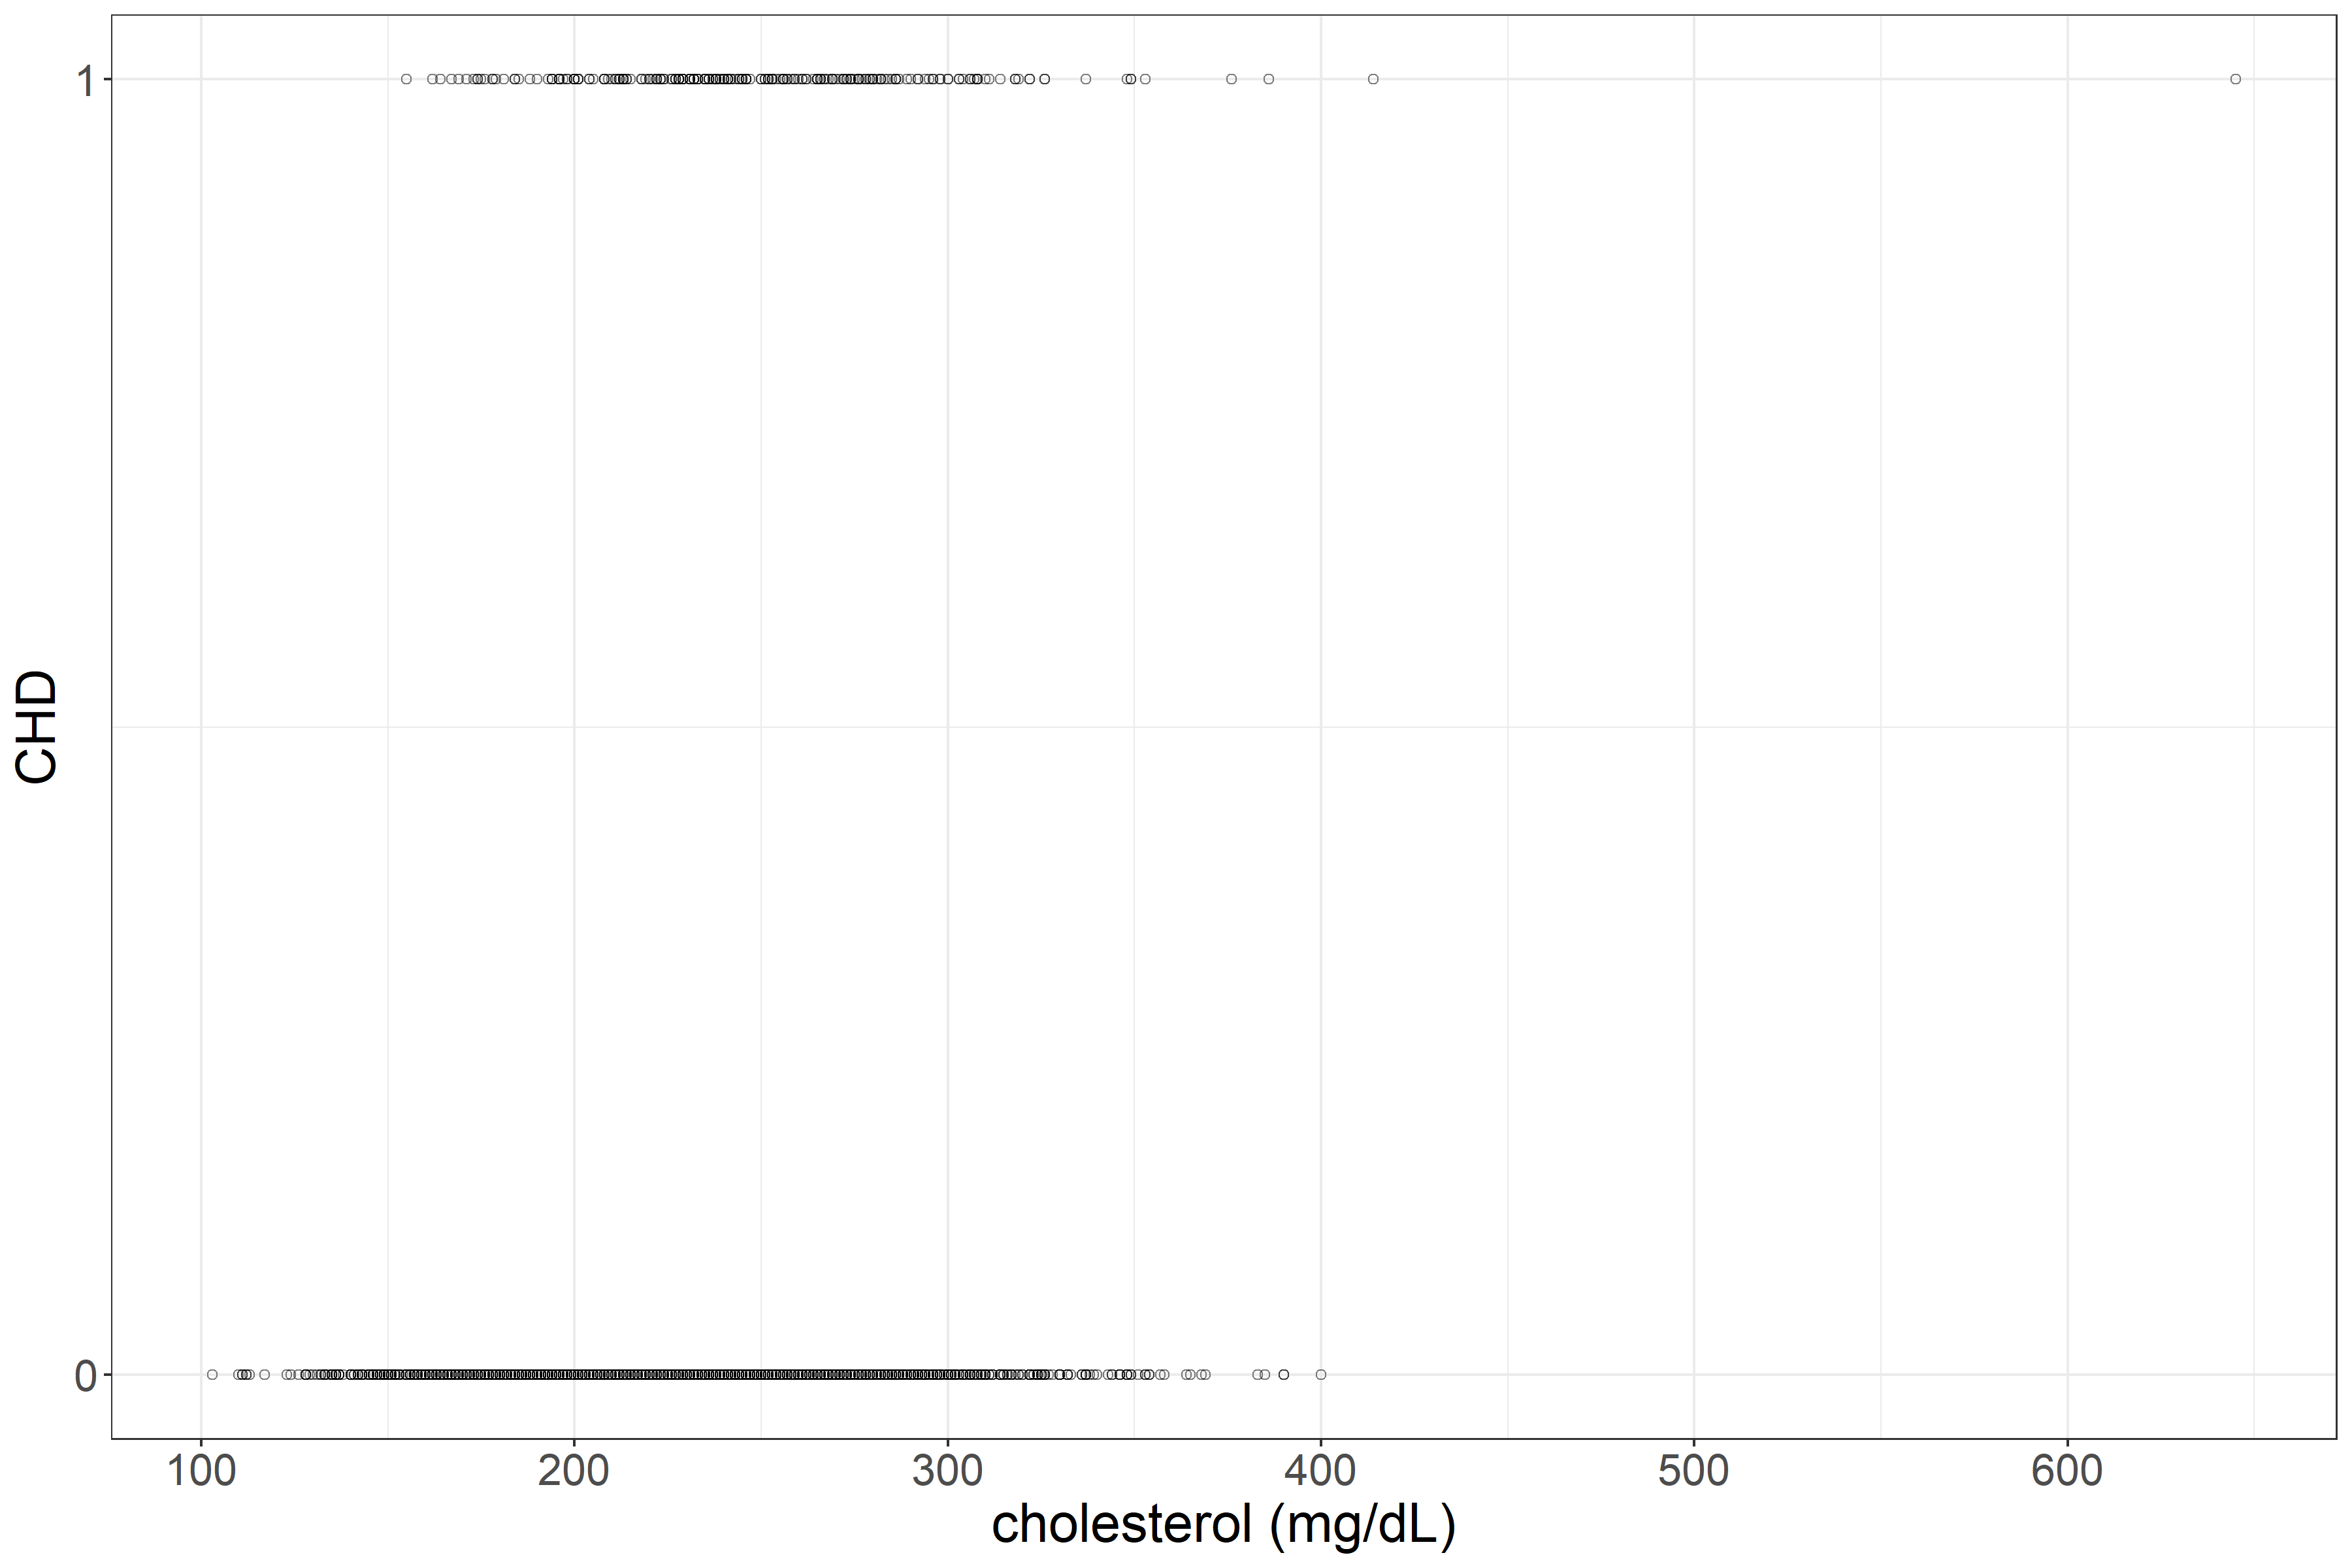
\includegraphics[width=0.7\textwidth]{./figs/scatter}
	\end{center}
\end{frame}

% graphical support: scatterplot
\begin{frame}{Linear regression with binary outcomes: Graphical support}
	We can plot the linear regression fit for this model.
	\begin{align*} 
		E[\texttt{chd}|\texttt{chol}] = \beta_0 + \beta_1 \texttt{chol}  
	\end{align*}
	
	\color{blue} Graphical support: \color{black} scatterplot with least squares line
	
	\begin{center}
		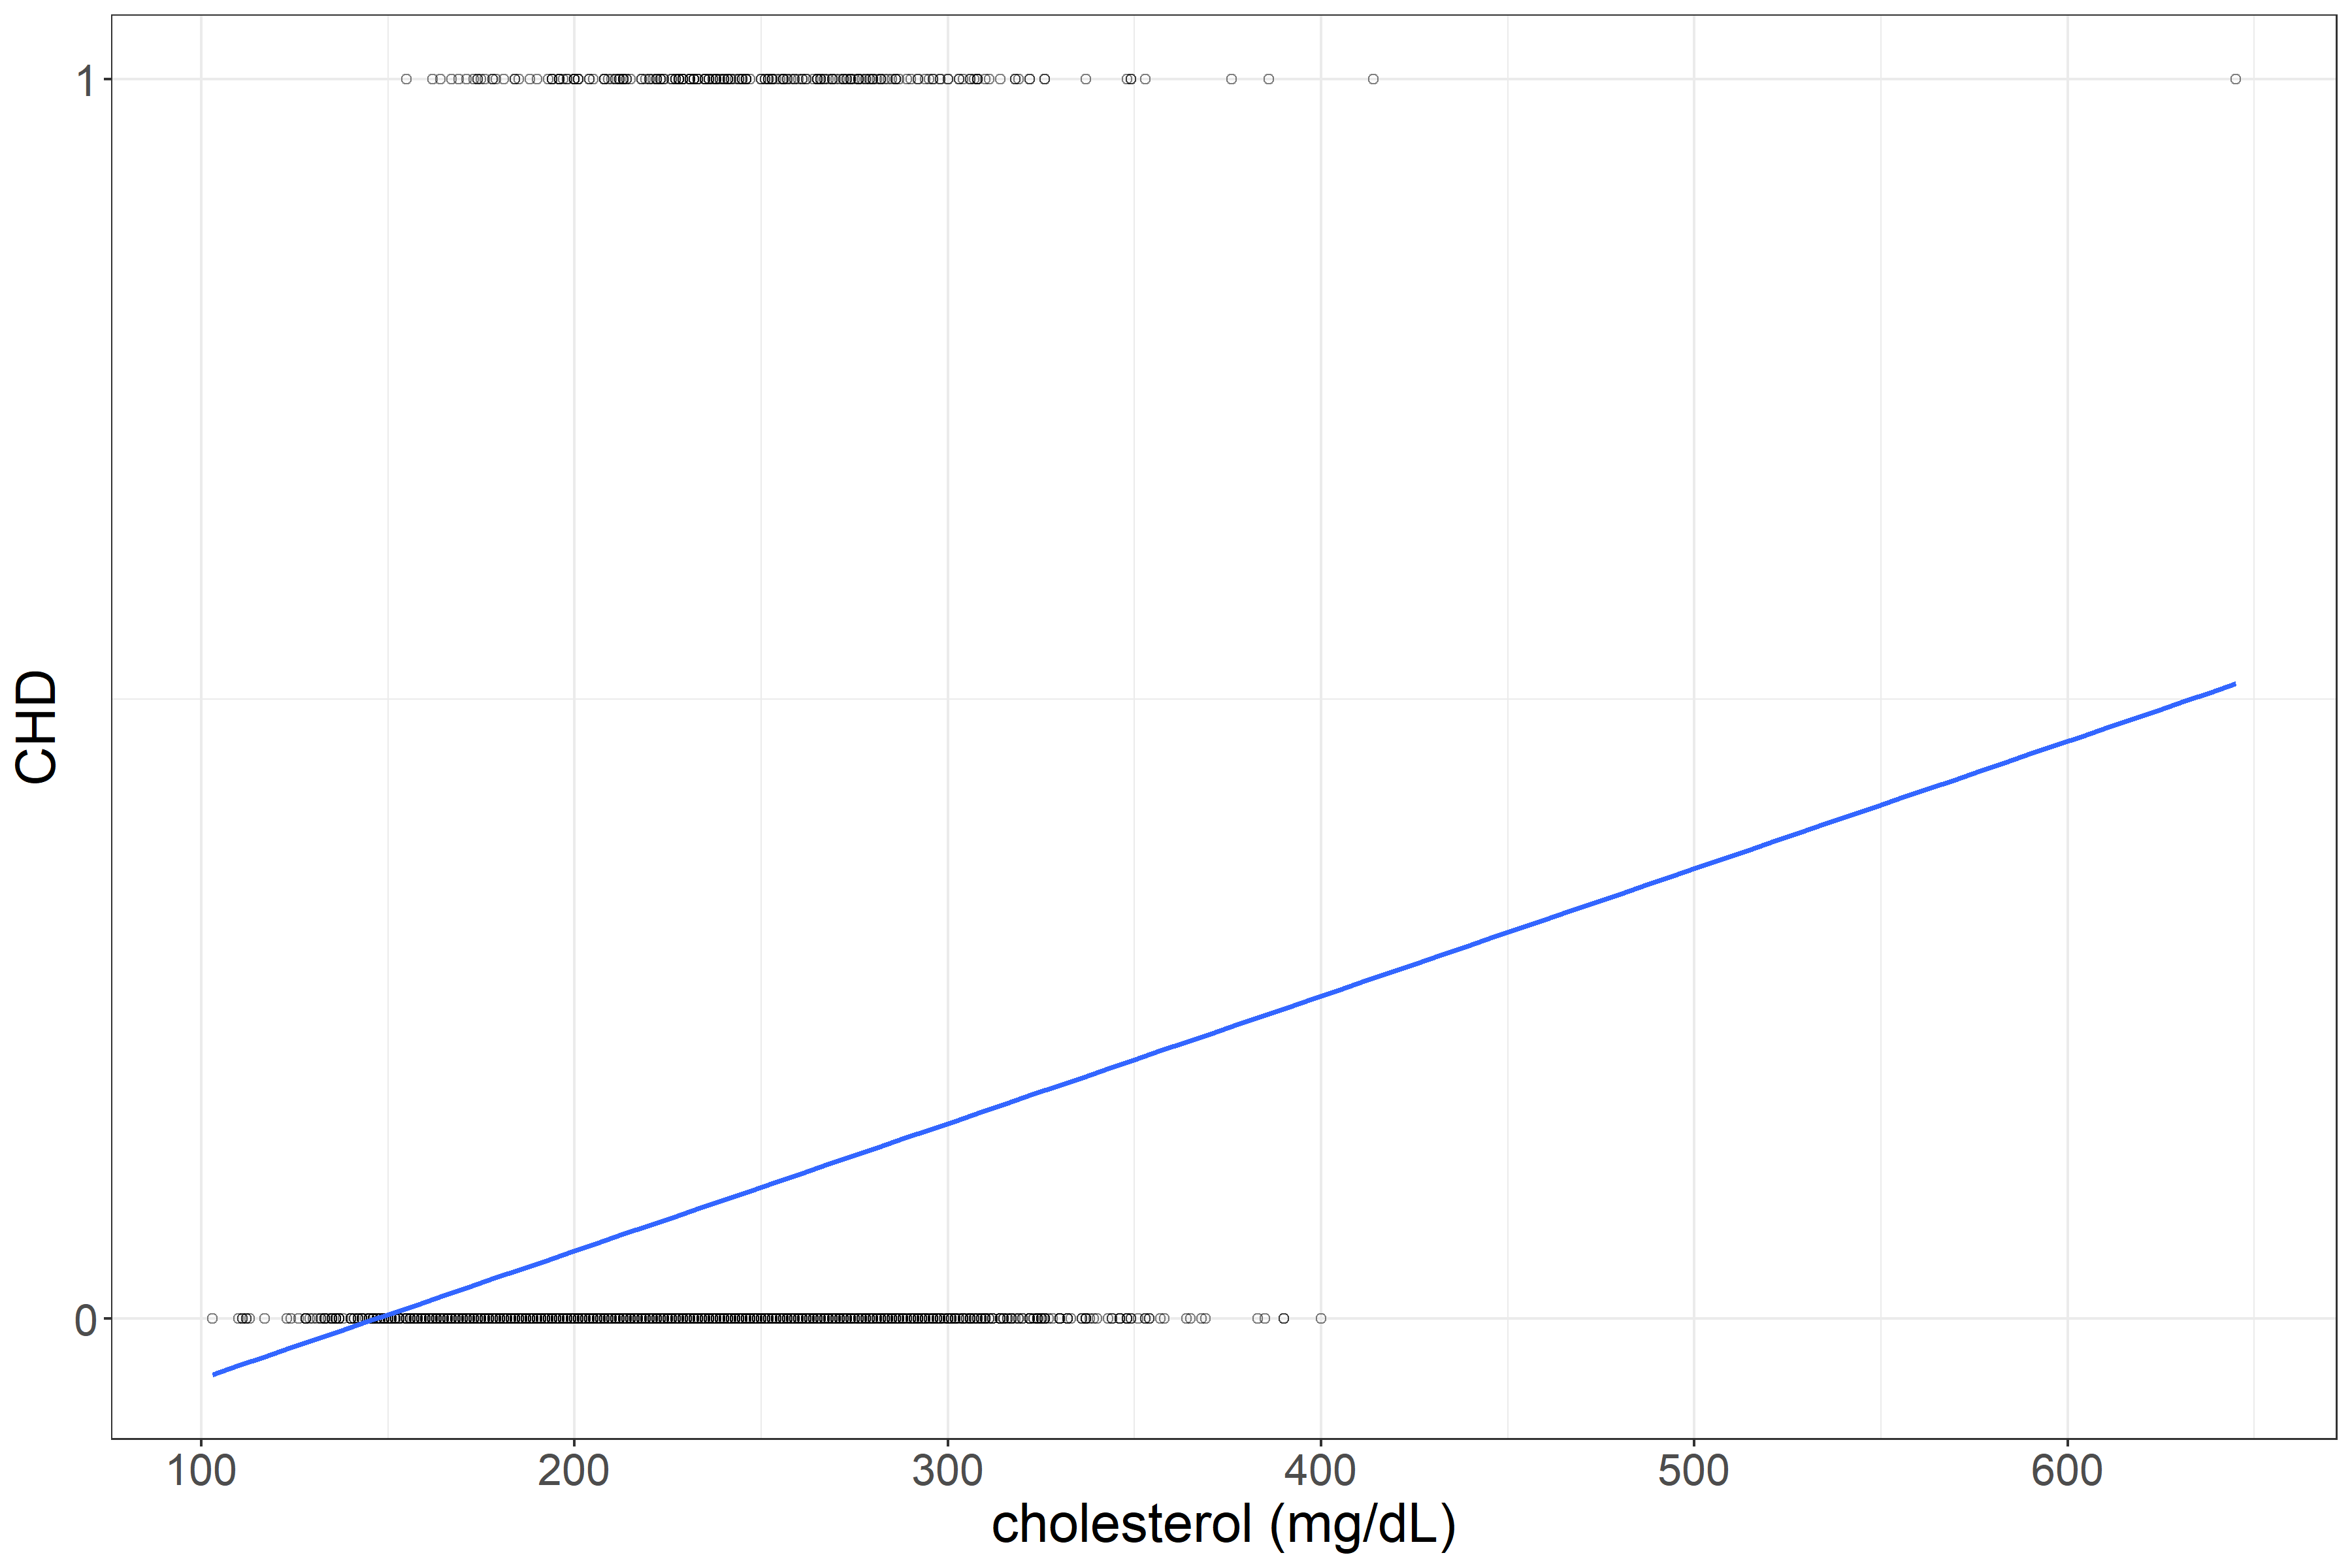
\includegraphics[width=0.7\textwidth]{./figs/scatter_lm}
	\end{center}
\end{frame}

\begin{frame}{Linear regression with binary outcomes: Graphical support}
	\vspace{-1cm}
	\begin{align*} 
		E[\texttt{chd}|\texttt{chol}] = \beta_0 + \beta_1 \texttt{chol}  
	\end{align*}
	What is the predicted probability of CHD for someone with cholesterol of 120 mg/dL?
	
	\begin{center}
		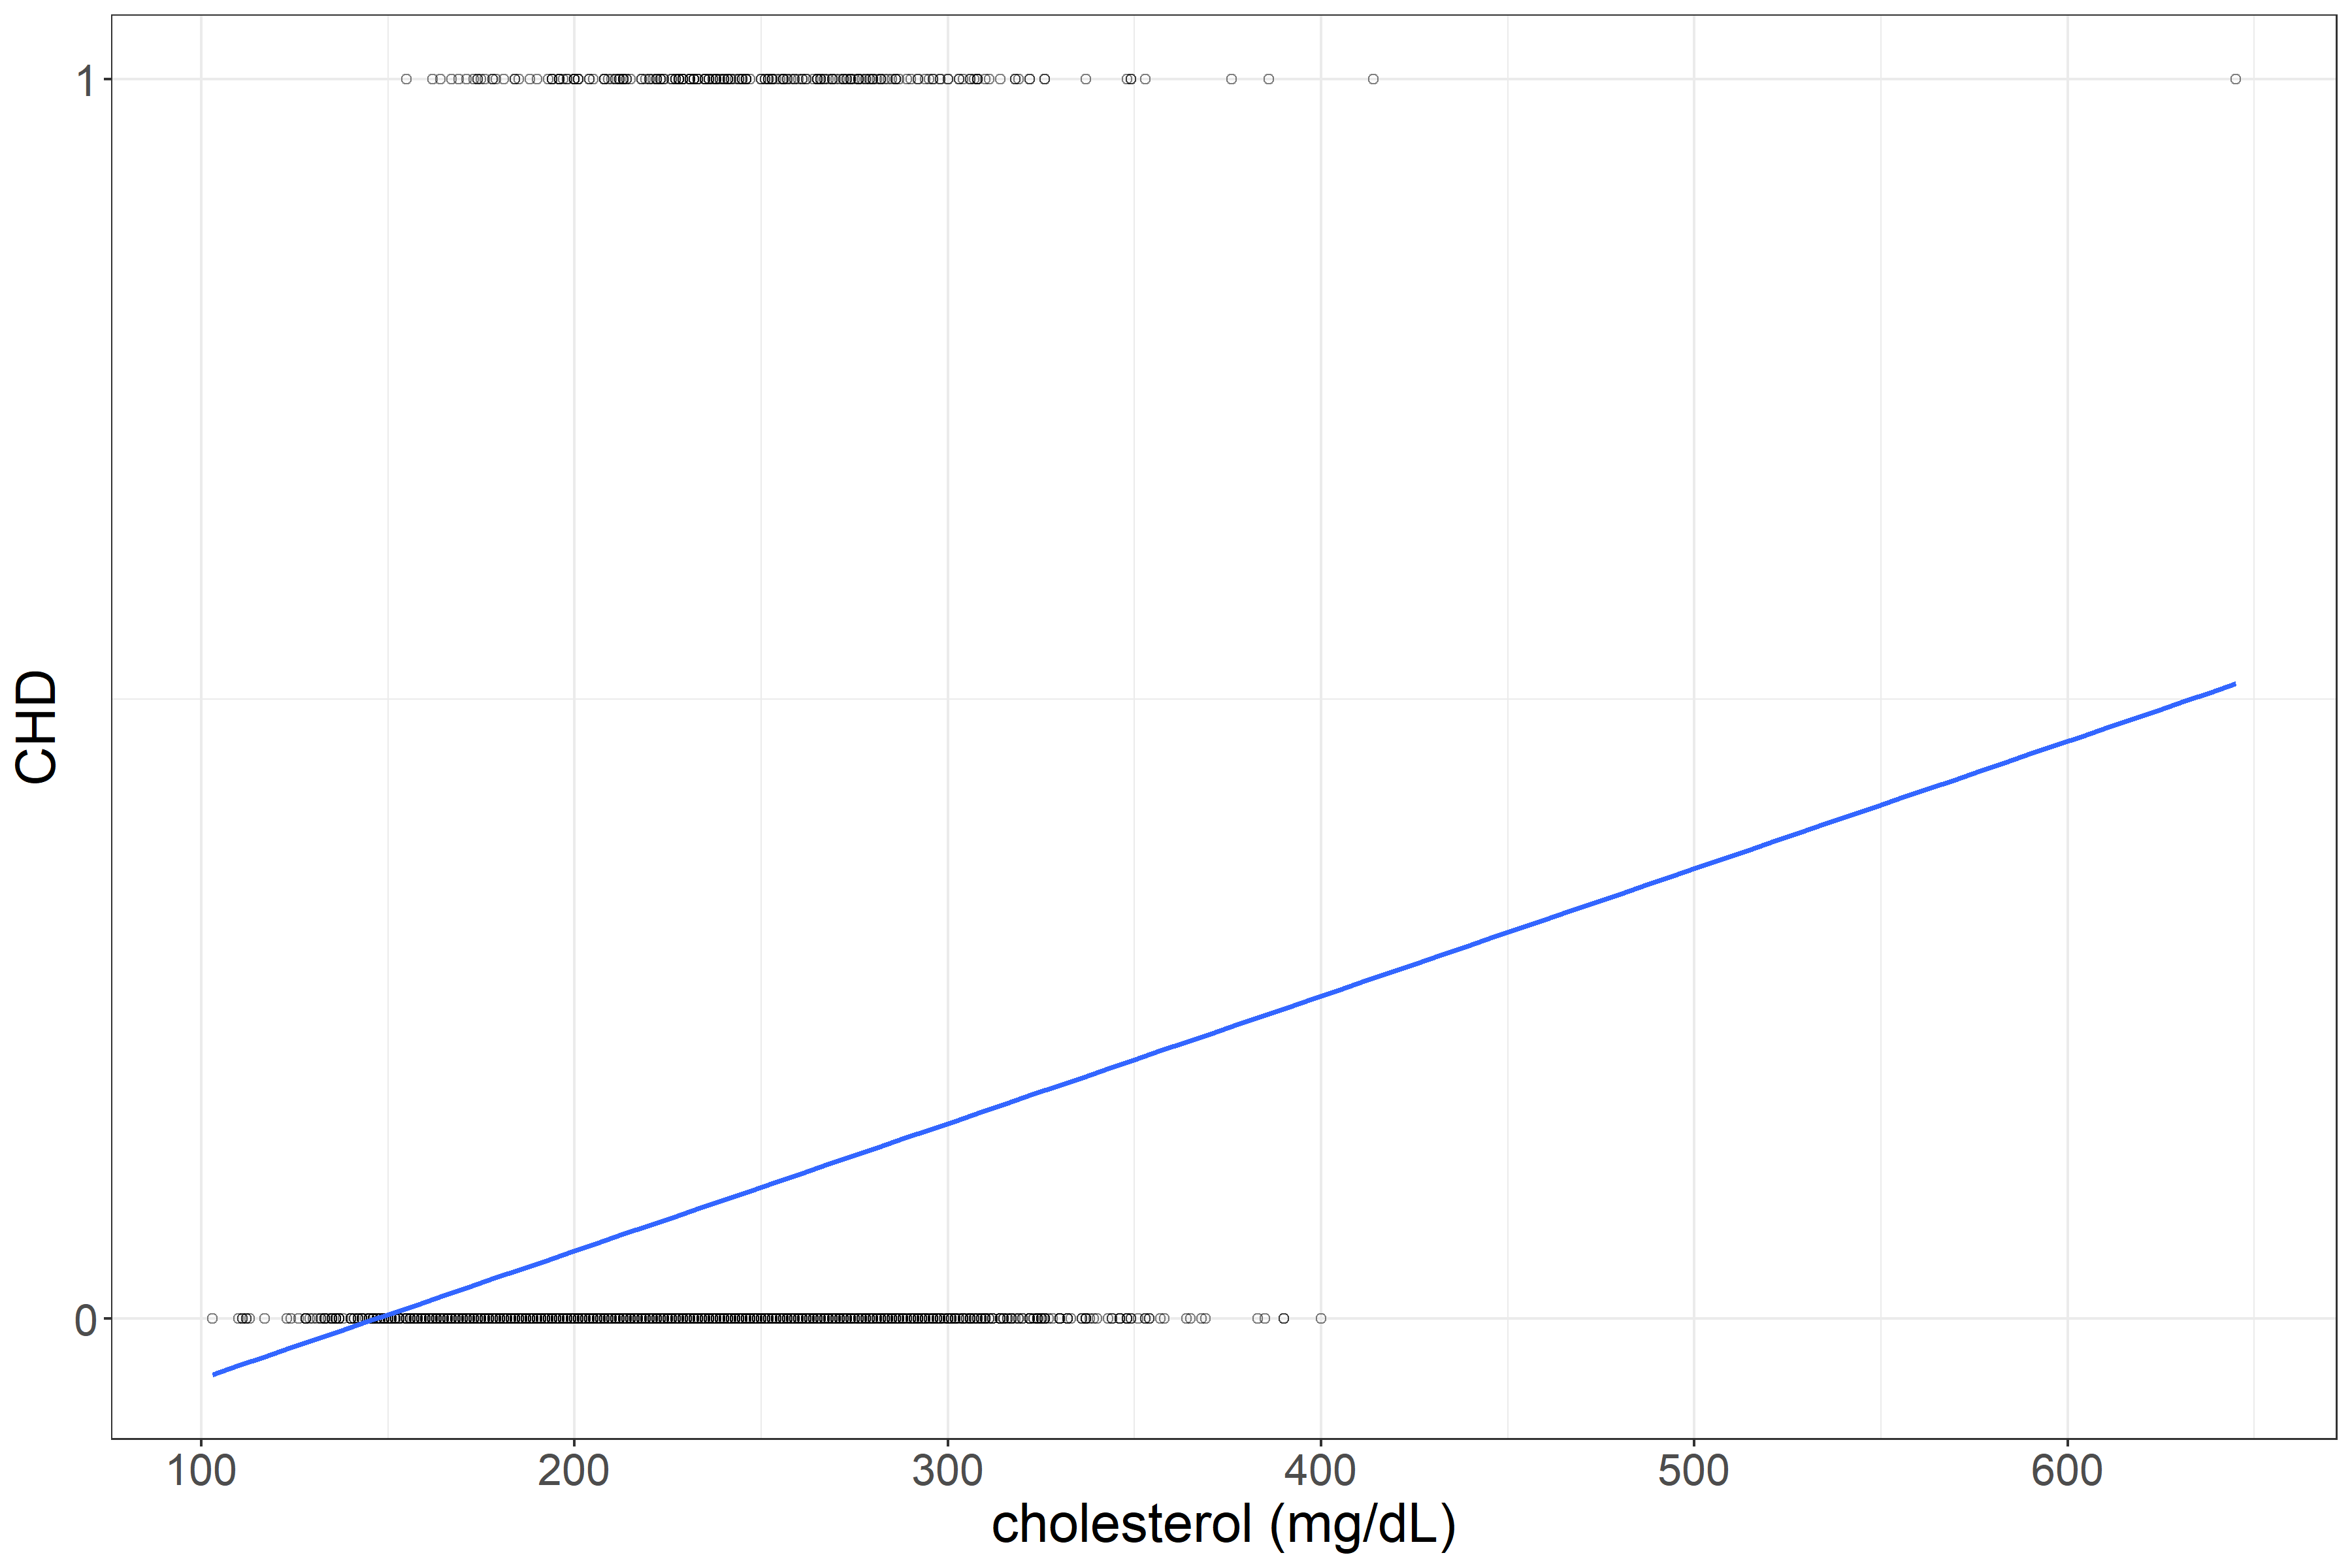
\includegraphics[width=0.7\textwidth]{./figs/scatter_lm}
	\end{center}
\end{frame}

\begin{frame}{Linear regression with binary outcomes: pros and cons}
	\vspace{-2cm}
	\begin{align*} 
		E[Y|X_1,\cdots,X_p] = \beta_0 + \beta_1 X_1 + \beta_2 X_2 + \cdots \beta_p X_p 
	\end{align*}
	
	Pros: 
	\begin{itemize}
		\item Easy to interpret (differences in probabilities)
	\end{itemize}
	
	Cons: 
	\begin{itemize}
		\item Predicted/fitted values can be outside the (0,1) range (as we just saw in the cholesterol example)
		\item Our mean model might not be correct (particularly the linearity assumption)% is one of the assumptions for linear regression that actually is important
	\end{itemize}
	
	What can we do instead?
\end{frame}


%\section{Simple logistic regression with binary outcome}
%% motivate logistic regression
%\begin{frame}
%	\frametitle{Diabetes vs sex: odds}
%	\begin{small} What if we wanted to quantify the association between diabetes and sex via the \textit{odds ratio} rather than the \textit{risk difference}? \end{small} \pause
%	
%	\vspace{-0.3cm}
%	
%	\begin{enumerate}
%		\item \textbf{Scientific Question:} is diabetes \textcolor{orange}{associated} with sex? \pause
%		\item \textbf{Statistical Question:} is the \textcolor{orange}{ratio of odds} of diabetes between men and women different from 1? \pause
%		\begin{itemize}
%			\item \textbf{Parameter:} odds ratio \pause
%		\end{itemize}
%		\item Take a \textbf{sample} from the population: cohort study of adults aged 65 and older from 4 US communities \pause
%		\item Perform \textit{statistical inference}:
%		\begin{itemize}
%			\item Calculate a corresponding \textbf{statistic}: sample odds ratio
%			\item Quantify uncertainty in your statistic
%			\item Perform a hypothesis test \pause
%		\end{itemize}
%	\end{enumerate}
%	
%	\vspace{-0.4cm}
%	We can use \textcolor{blue}{logistic} regression to answer this question!
%\end{frame}
%
%
%
%
%% ask them to think about logistic regression interp
%\begin{frame}
%	\frametitle{Activity (continued): diabetes vs sex}
%	Suppose we fit the logistic regression model $$\log\left(\text{Odds}[diabetes | male]\right) = \beta_0 + \beta_1 male$$
%	
%	\color{blue} On the same piece of paper, please answer these questions:
%	
%	\begin{enumerate}
%		\item[3.] \color{blue} Interpret the intercept, $\beta_0$.
%		\item[4.] Interpret the slope, $\beta_1$.
%	\end{enumerate}
%\end{frame}
%
%% logistic regression: diabetes vs sex
%\begin{frame}
%	\frametitle{Logistic regression: diabetes vs sex}
%	
%	Suppose we fit the logistic regression model $$\log\left(\text{Odds}[diabetes | male]\right) = \beta_0 + \beta_1 male$$
%	
%	\vspace{-0.2cm}
%	
%	How do we interpret the regression coefficients $\beta_0, \beta_1$? \vspace{-0.3cm}
%	\begin{itemize}
%		\item $\beta_0$: \pause the log odds of diabetes among females \pause
%		\item[] \color{blue} $e^{\beta_0}$: the odds of diabetes among females \pause \color{black}
%		\item $\beta_1$: \pause the difference in log odds of diabetes between males and females \pause 
%		\item[] \color{blue} $e^{\beta_1}$: the ratio of odds between males and females \color{black}
%	\end{itemize}
%	
%	\vspace{-0.2cm}
%	To answer our statistical question \begin{small}\textit{(is the ratio of odds of diabetes between men and women different from 1?)}\end{small} we just need to look at $e^{\beta_1}$! \begin{small} (estimate, CI, test if it's equal to 1) \end{small}
%\end{frame}
%
%\begin{frame}
%	The interpretation of logistic regression models is
%	\begin{itemize}
%		\item[] \color{blue} more complicated \color{black} (we have to remember to exponentiate the coefficients, and to talk about ratios rather than differences), and
%		\item[] \color{orange} less intuitive \color{black} (a lot of people don't understand the difference between probabilities and odds)...
%	\end{itemize}
%	\textit{so why bother?}
%\end{frame}
%



\section*{References}
\begin{frame}
% to enforce entries in the table of contents
\end{frame}

\end{document}